\documentclass{article}

%%% Load packages
%\usepackage{amsthm,amsmath}
%\RequirePackage{natbib}
%\RequirePackage[authoryear]{natbib}% uncomment this for author-year bibliography
%\RequirePackage{hyperref}
\usepackage[utf8]{inputenc} %unicode support
%\usepackage[applemac]{inputenc} %applemac support if unicode package fails
%\usepackage[latin1]{inputenc} %UNIX support if unicode package fails
\usepackage{geometry} %margins
\geometry{top=27mm} \geometry{bottom=17mm} \geometry{left=2cm}
\geometry{right=2cm}
%\usepackage[section]{placeins}
\usepackage{textcomp} \usepackage{textgreek} %\usepackage{adjustbox}
%\usepackage{enumitem} \setlist{itemsep=2pt,parsep=4pt,topsep=2pt,partopsep=4pt}
%\usepackage[small]{caption}
\usepackage[colorlinks=true,urlcolor=blue,citecolor=blue,linkcolor=blue]{hyperref} %\usepackage[dvipsnames]{xcolor} %for custom colors
%
%\usepackage{tikz} %for the colored bar
%fonts
%\usepackage{lmodern}
%\usepackage{newtxtext,newtxmath}
%\usepackage[letterspace=160,babel=true,tracking=true,kerning=true]{microtype}

%Bibliography
%% !BIB TS-program = biber
%\usepackage{csquotes}
%\usepackage[backend=biber,style=authoryear,useauthor=true,uniquename=false,natbib]{biblatex} 
%\addbibresource{references.bib}

%better control of floats
\usepackage{graphicx}
\usepackage{float,caption}
\renewcommand{\thefigure}{S\arabic{figure}}

%\makeatletter \patchcmd{\@maketitle}{\LARGE}{\Large}{}{} \makeatother

%\usepackage{titlesec} % % %\titleformat{\title}{\tiny}{\thetitle}{1em}{}
%\titleformat{\chapter}
%  {\normalfont\Large\bfseries}{\thechapter}{1em}{}
%\titlespacing*{\chapter}{0pt}{3.5ex plus 1ex minus .2ex}{2.3ex plus .2ex}
%\titleformat{\section}{\Large\bfseries}{\thesection}{1em}{}



\newcommand{\cit}{\colorbox{pink}{[reference?]}}
\newcommand{\mcit}{\colorbox{cyan}{[reference!]}}

%item labels
\renewcommand{\labelitemi}{$\circ$}


%%% Begin ...
\begin{document}
	
\title{Supplemental Figures} %%for... title
\author{Drozdova \textit{et al.}} %% all authors
%%\date if need a fixed date
\maketitle

\section{Diversity of opsin transcripts and their phylogenetic distribution}

\begin{figure}[H] 
\hskip -1cm 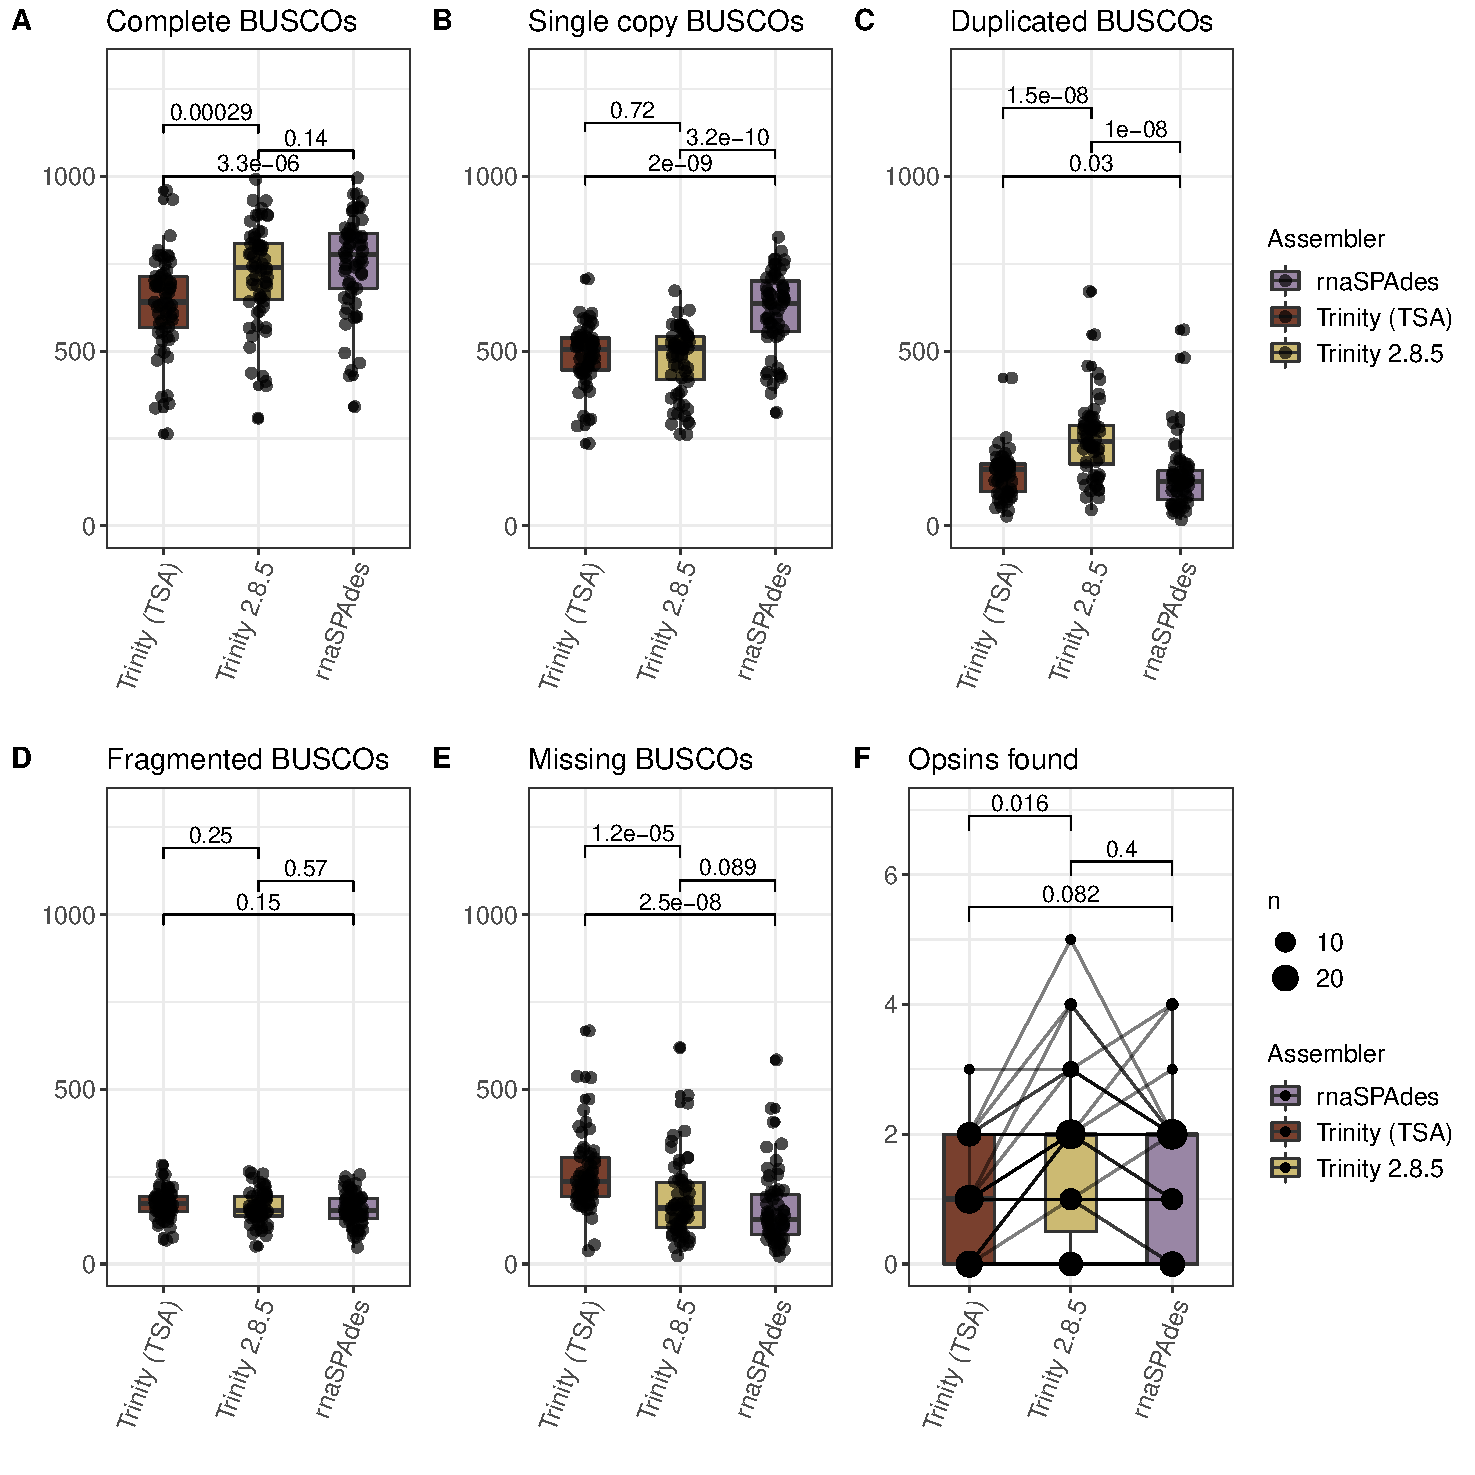
\includegraphics[scale=0.8]{./FigS1_assembly_comparison.pdf}
	\caption{Quality of transcriptome assemblies according to BUSCO metrics (A-E)} and the number of opsins found in each assembly (F). \end{figure}

\begin{figure}[H] 
	\vskip -18mm
	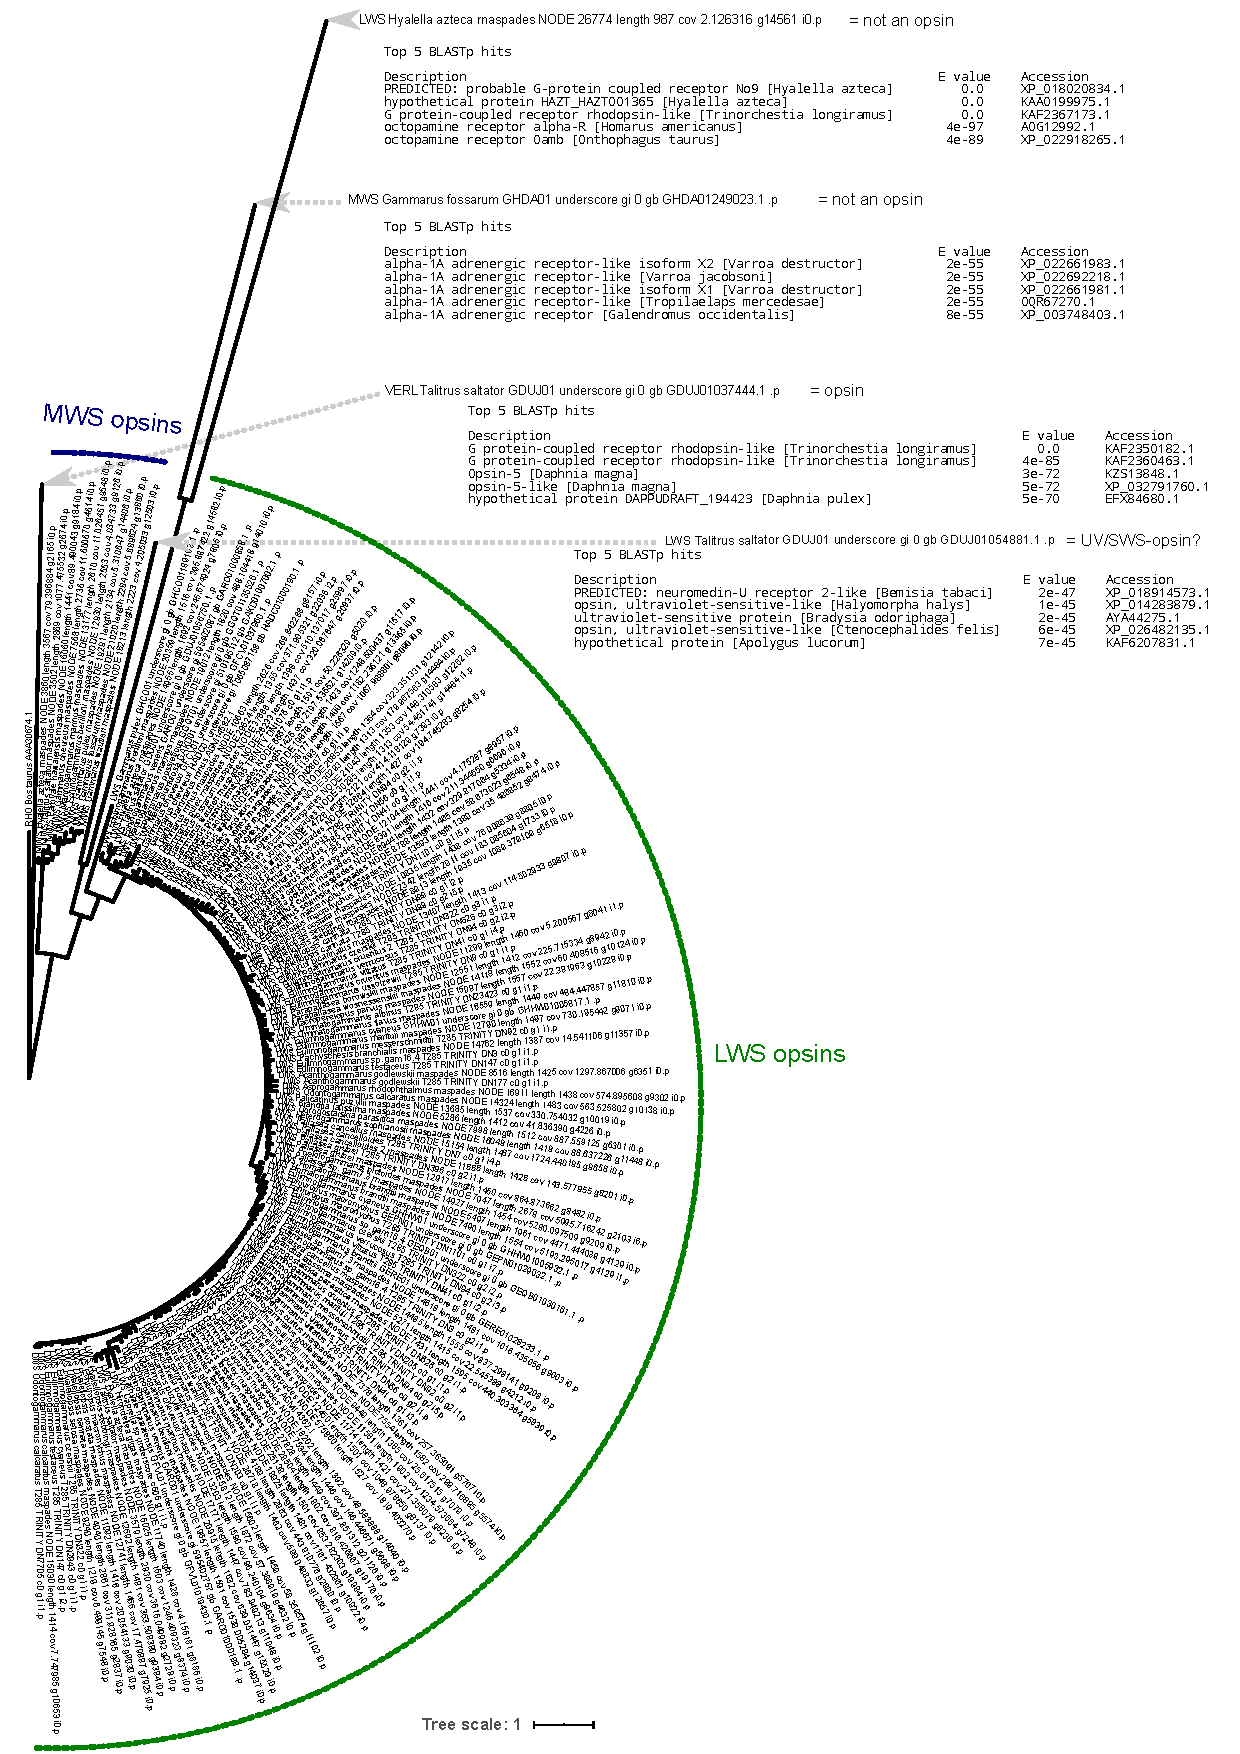
\includegraphics[scale=0.85]{FigS2a_opsin_tree.pdf}
	\caption{(A) An amino acid-based maximum likelihood tree of all found opsin sequences and reanalysis of long branches with NCBI BLAST.} 
\end{figure}

\begin{figure}[H] 
	\ContinuedFloat
	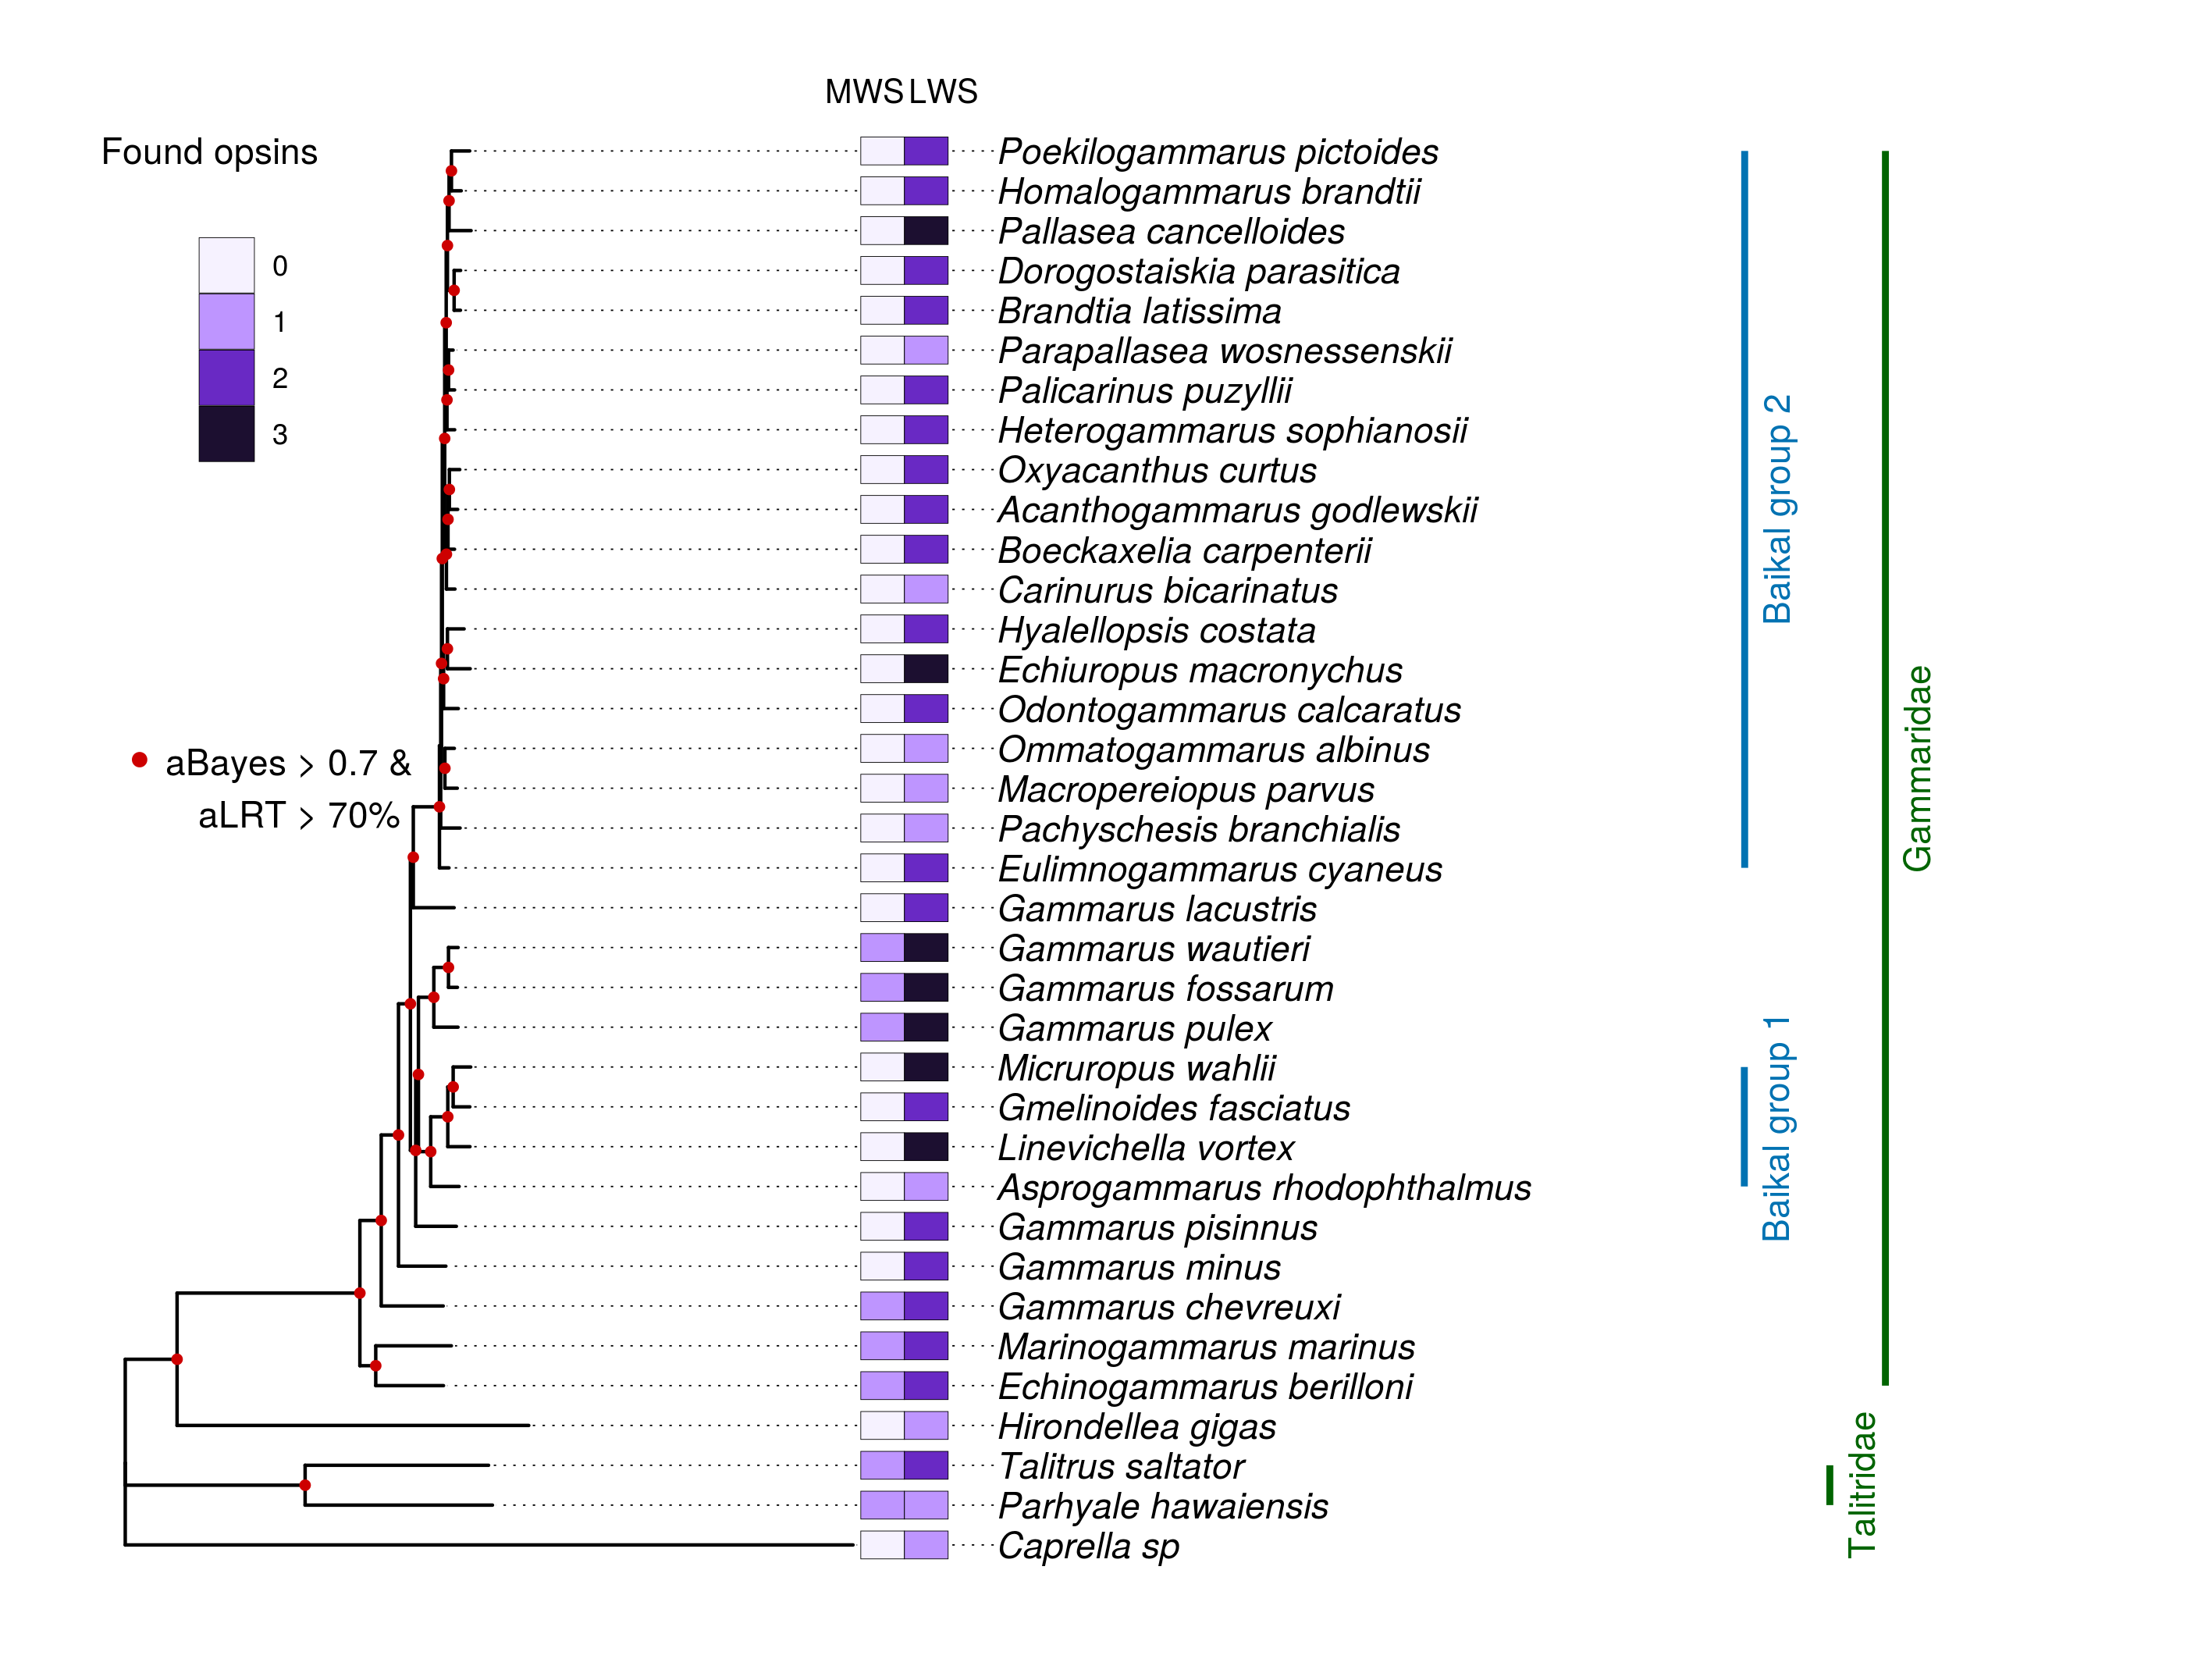
\includegraphics[scale=0.85]{FigS2_aa_tree.png}
	\caption{(B) Amino acid-based species tree based on one-copy orthologous proteins.} 
\end{figure}


\begin{figure}[H] 
	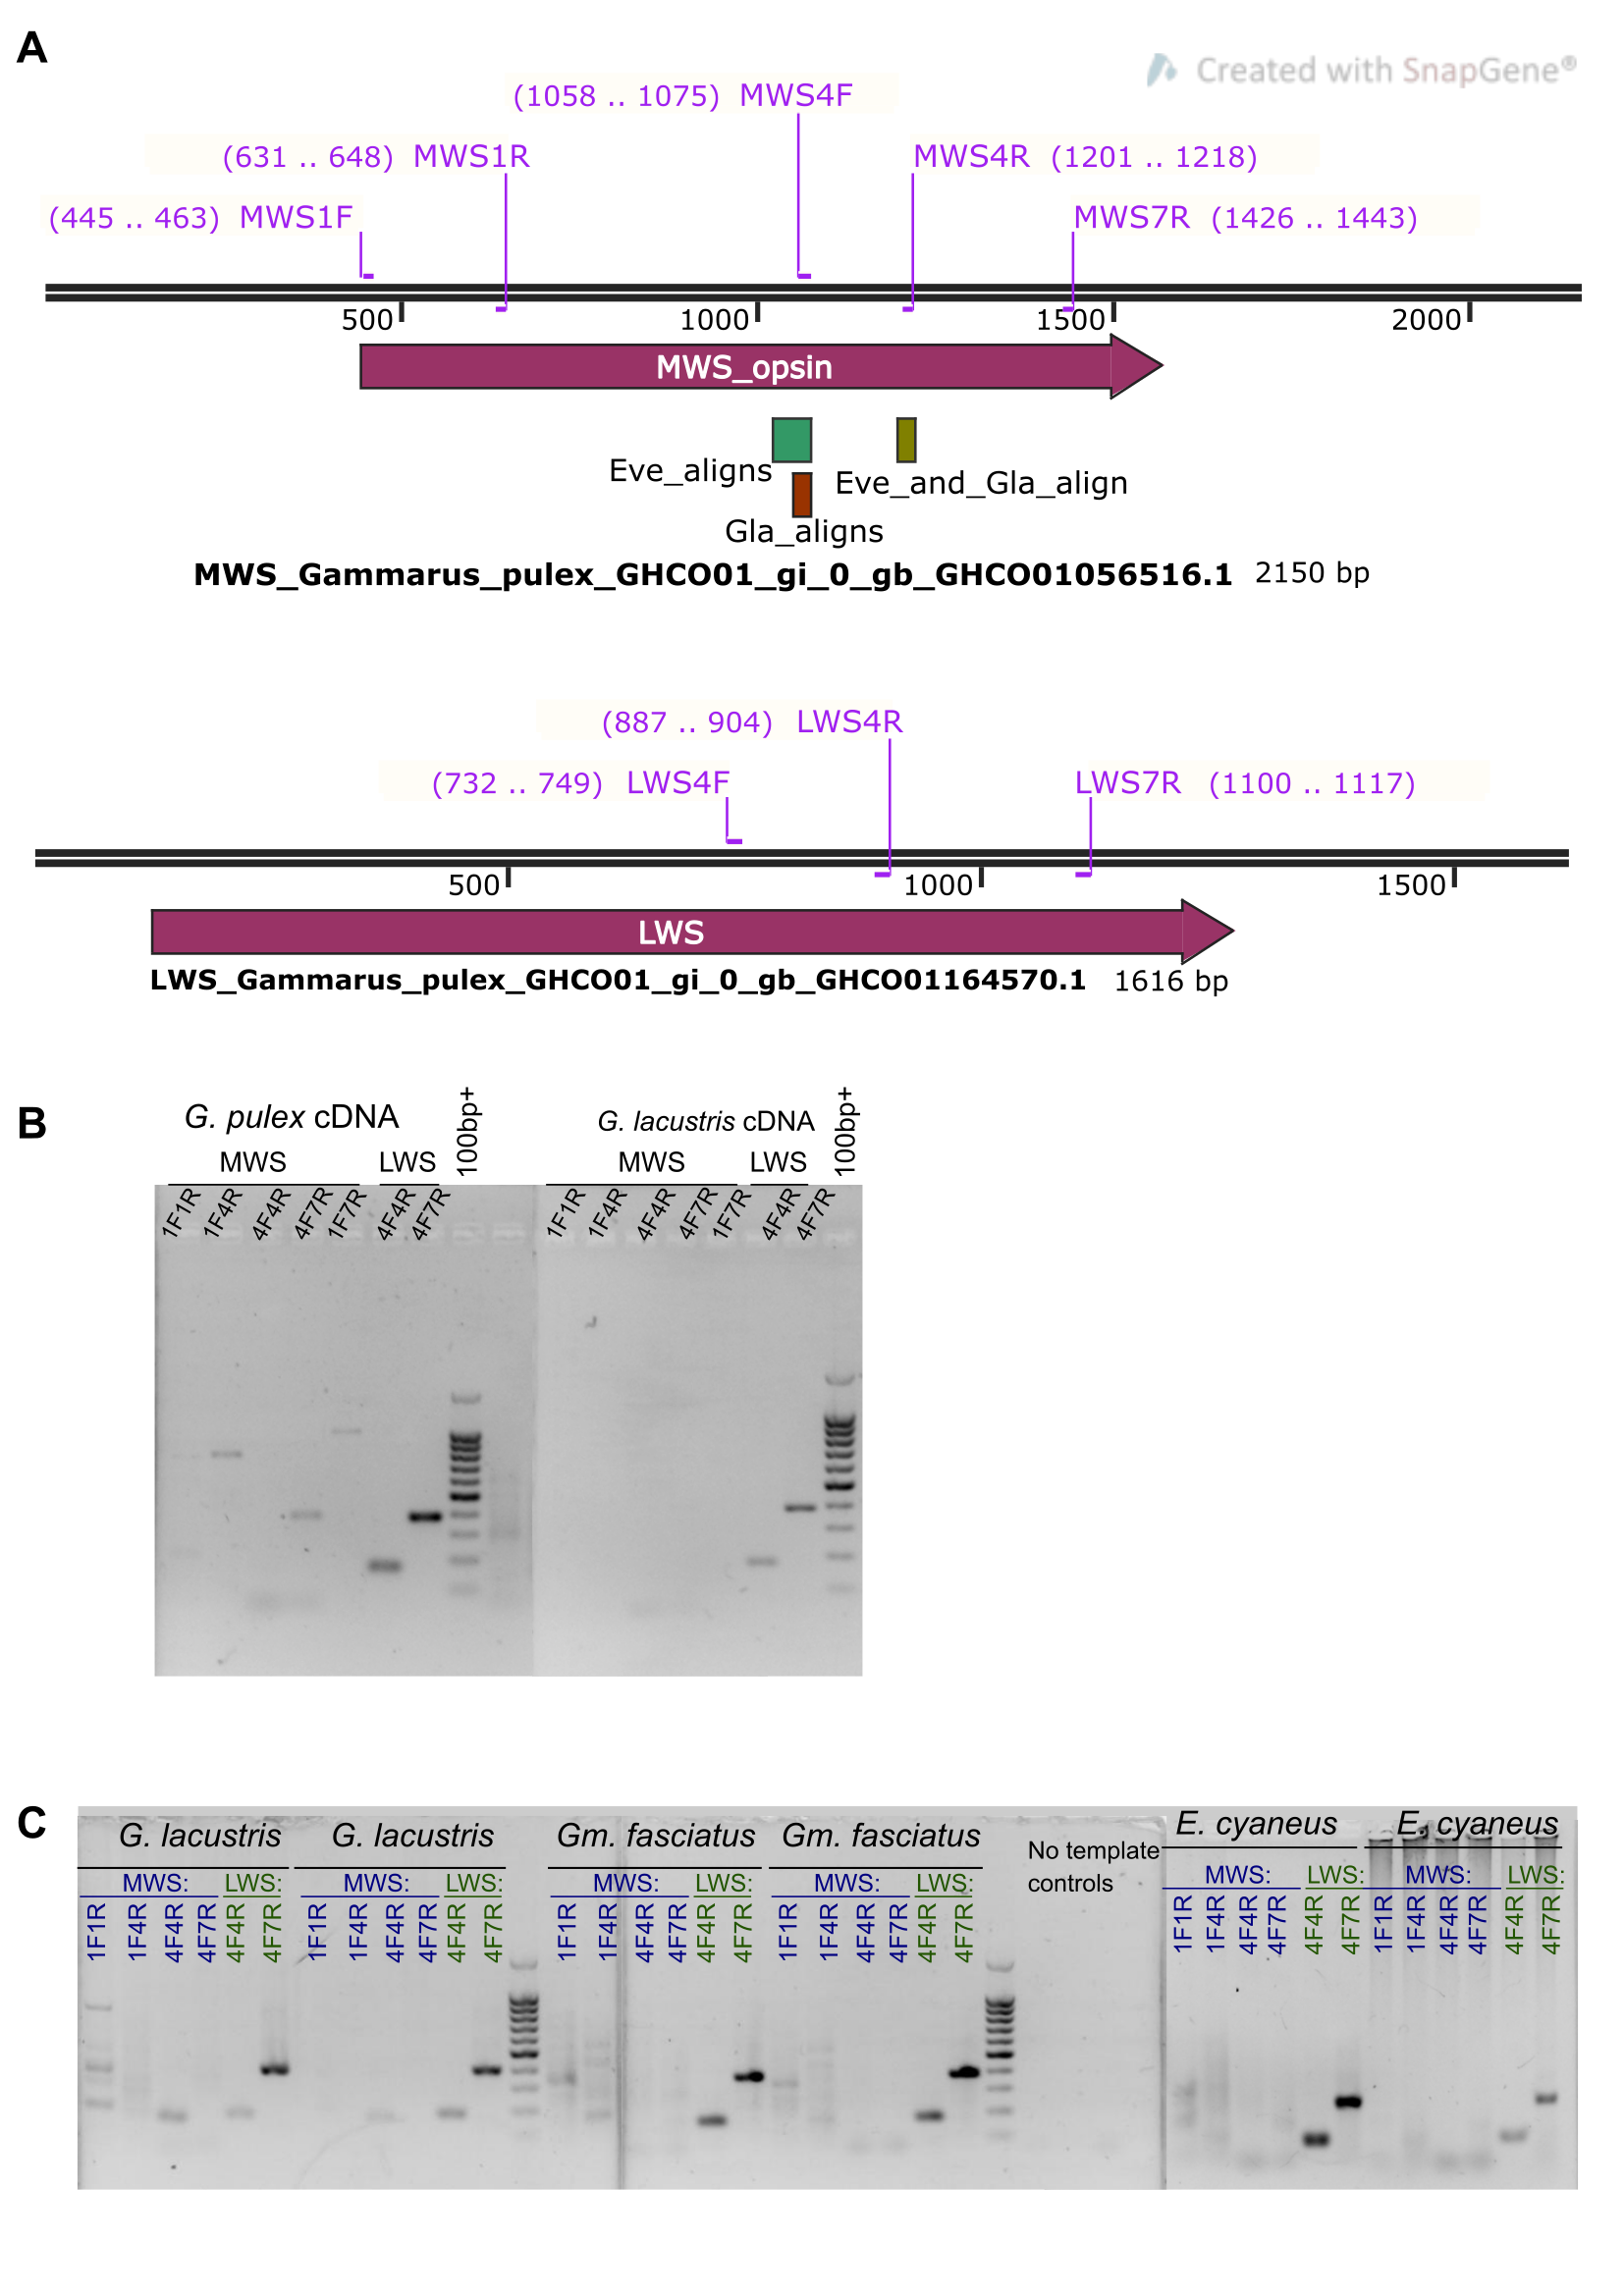
\includegraphics[scale=0.75]{./FigS3_gDNA_PCR_Gmfa_Ecy_Gla.png}
	\caption{Amplification of MWS and LWS opsins from extracted genomic DNA of several species. (A) Schematic of primer binding sites. (B) Opsin amplification from \textit{G. pulex} and \textit{G. lacustris} cDNA. (C) Opsin amplification from genomic DNA of several species.} \end{figure}

\begin{figure}[H] 
	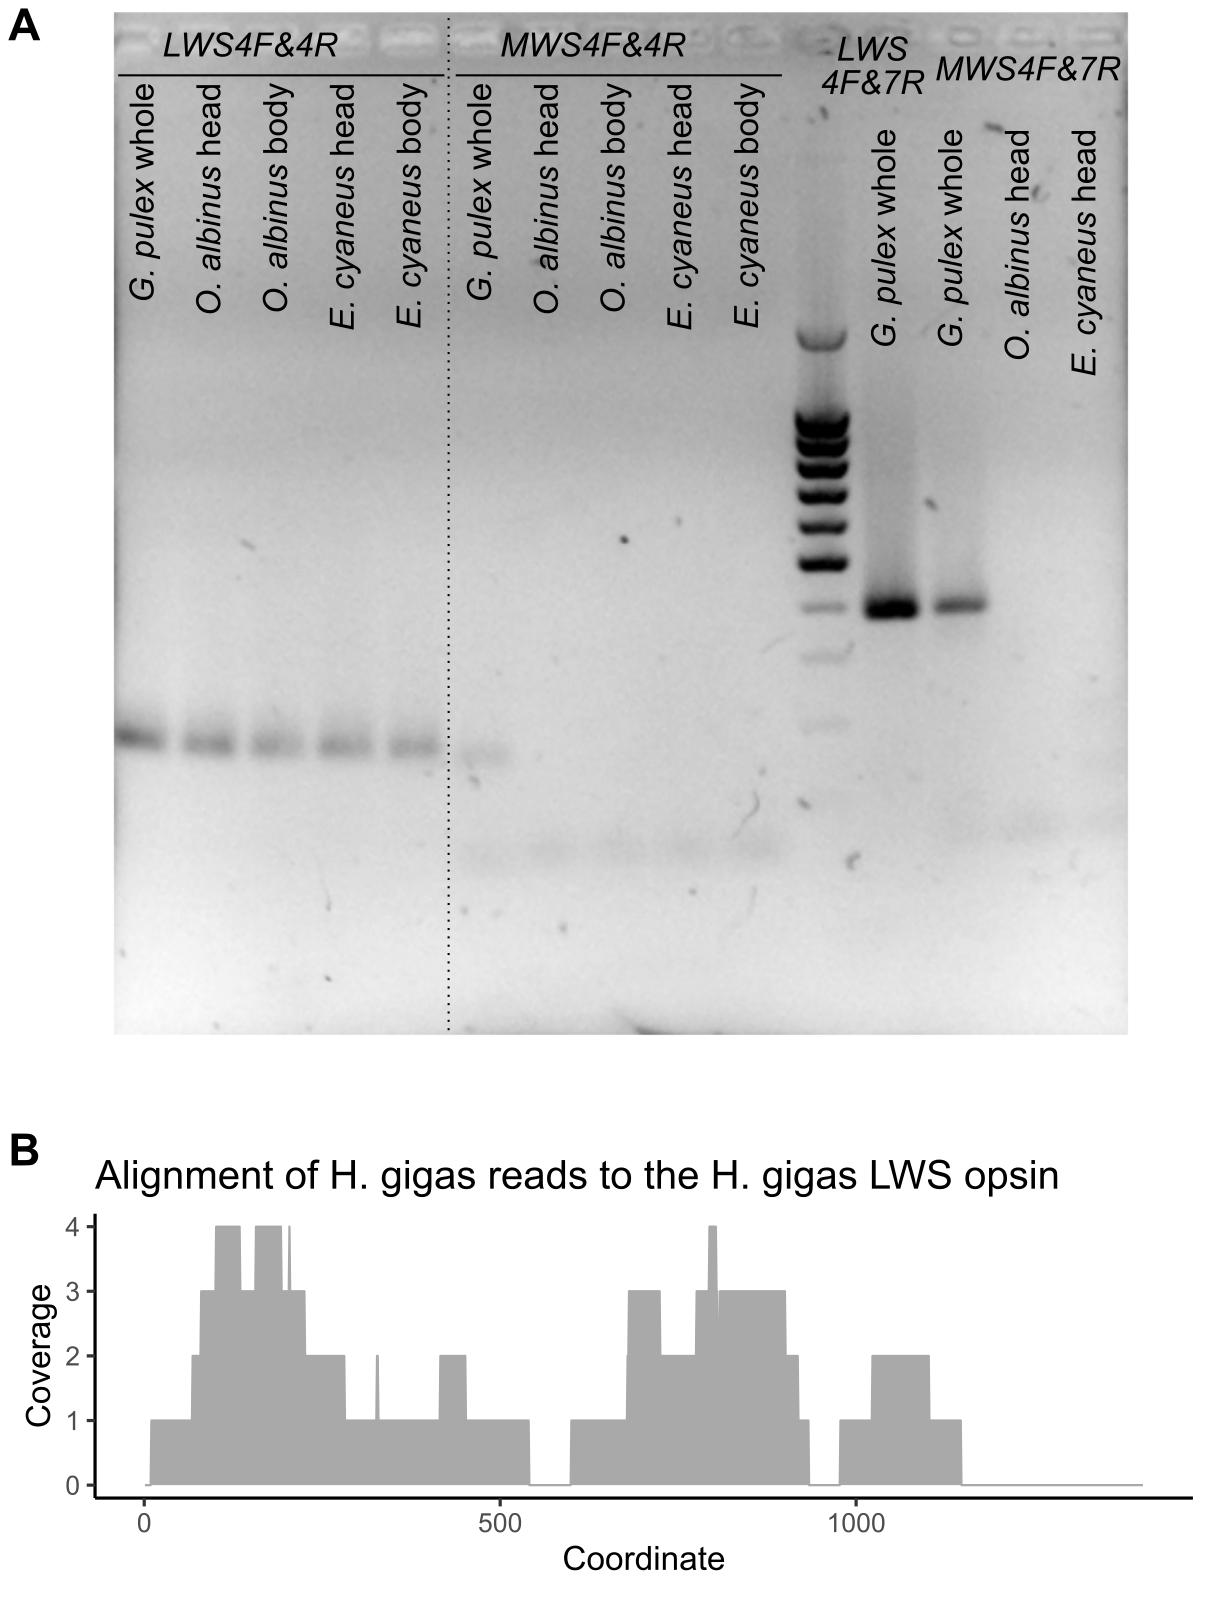
\includegraphics[scale=0.65]{./FigS4_cDNA_diff_body_parts.png}
	\caption{Evidence for extraocular expression of opsins in amphipods. (A) Opsin amplification from cDNA of several species. (B) Expression of the \textit{H. gigas} LWS opsin in the sample from pereon and pleon.} \end{figure}

\begin{figure}[H] 
	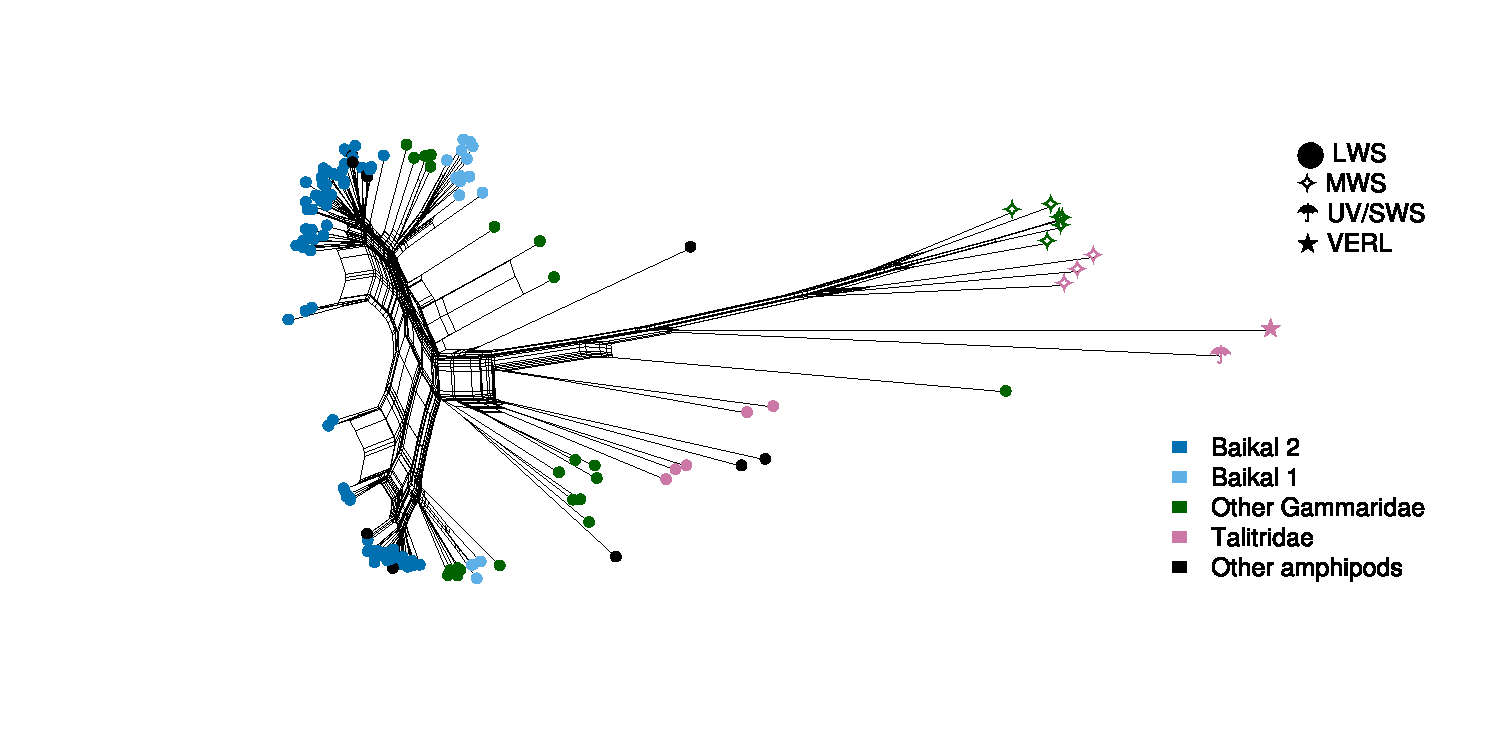
\includegraphics[width=\linewidth]{./FigS5_all_opsins_network.pdf}
	\caption{Phylogenetic network of all found amphipod opsins based on nucleotide sequences.} \end{figure}

\begin{figure}[H] 
	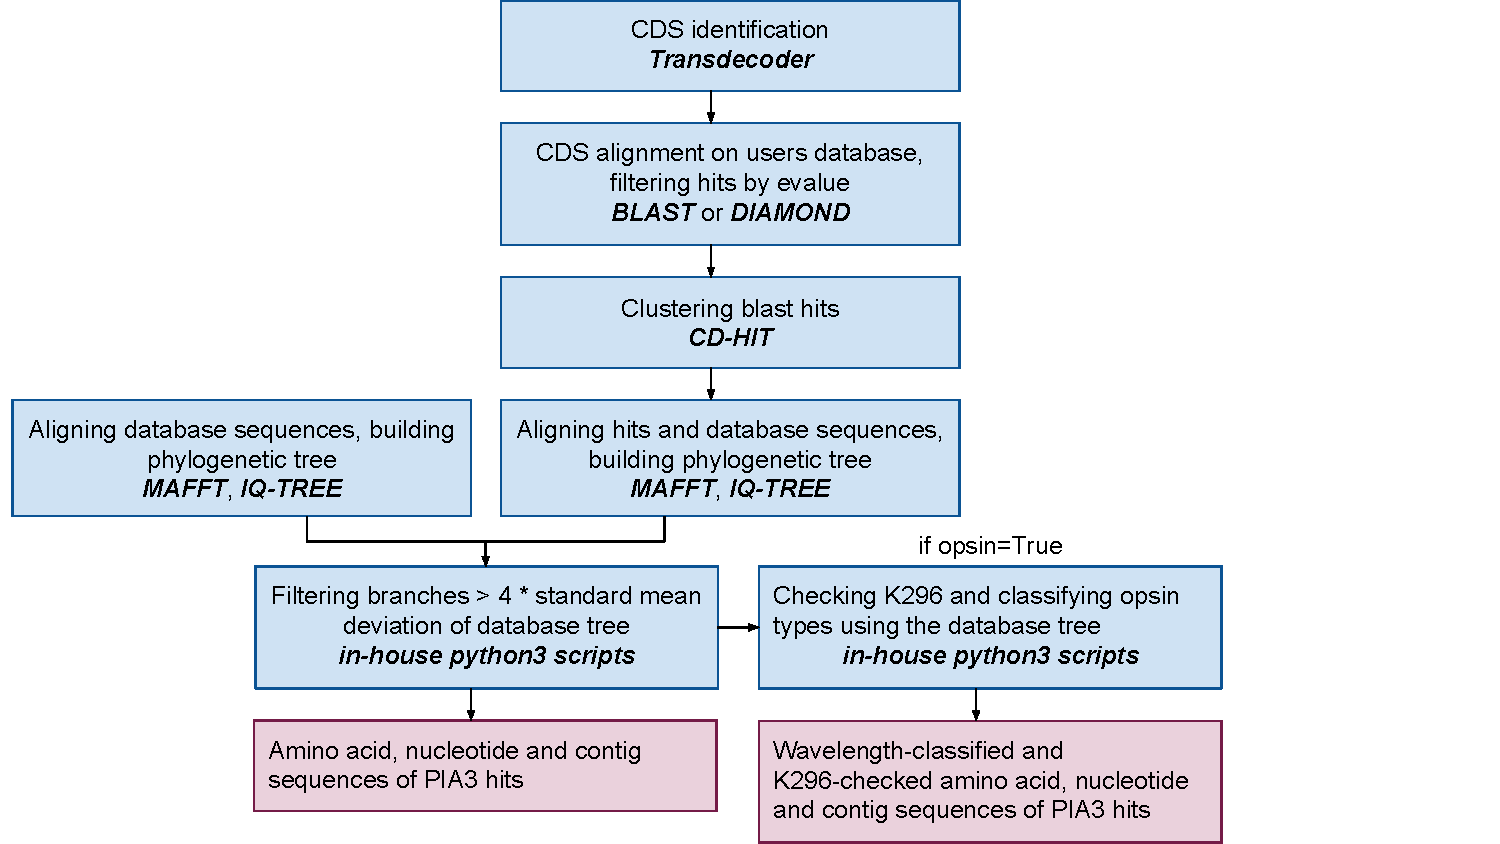
\includegraphics[width=\linewidth]{./FigS6_PIA3.pdf}
	\caption{PIA principle.} \end{figure}


\begin{figure}[H] %
	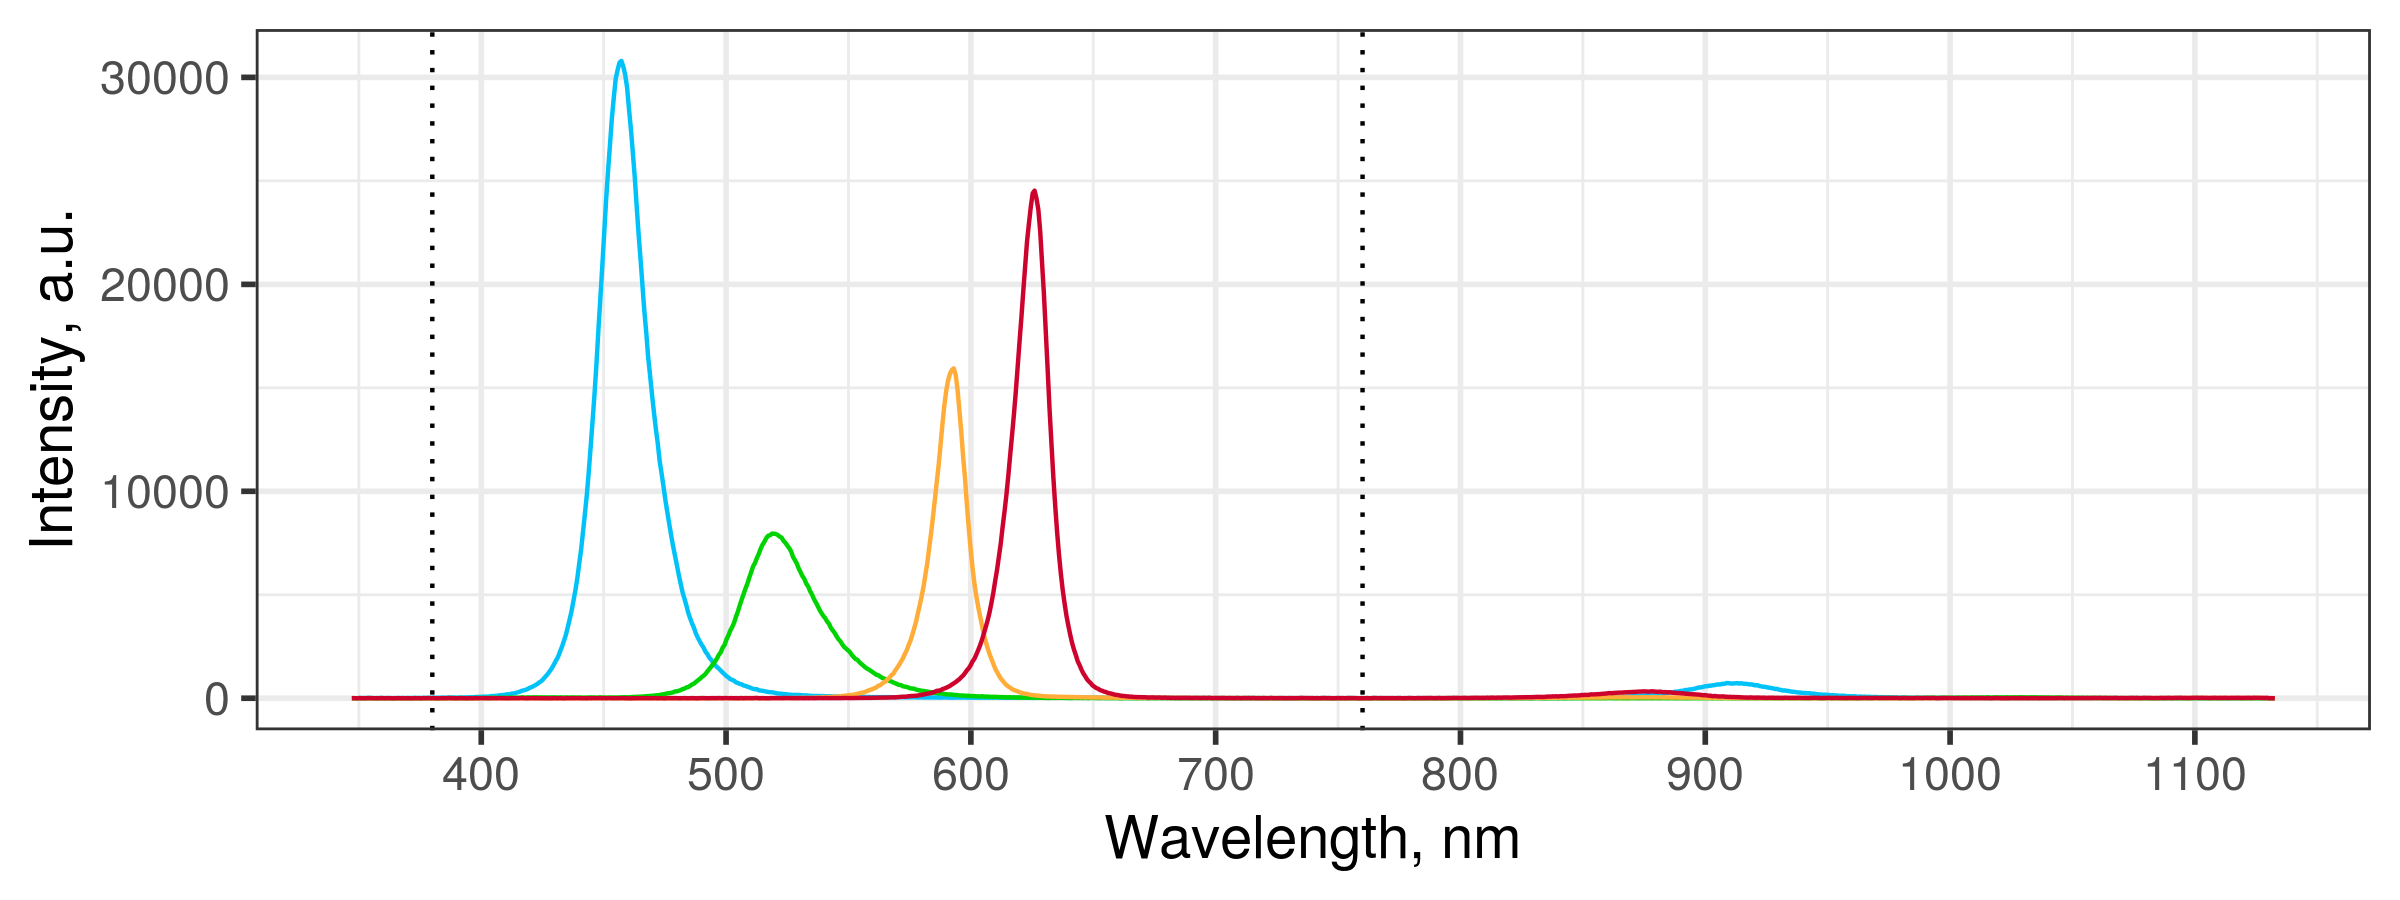
\includegraphics[width=\linewidth]{./FigS7_spectra.png}%
	\caption{Emission spectra of the LED light sources.} \end{figure}

	
\end{document}

